% U-Speak ウェブ版・島とゲームの説明書
%
% 教室さま（とくに U-Speak Roblox をすでに使っている教室さま）にお渡しする資料です。
% 画像は docs/figures/ の PNG（server/test/e2e/capture-figures.mjs が撮ったもの）。
%
%   組む:  cd docs && xelatex uspeak-guide.tex  （2回。目次と図番号のため）
%
% 日本語を組むので XeLaTeX を使います（LuaLaTeX 用の前置きにはなっていません）。
% 保護者レポート（server/src/game/report-tex.js）と同じ色・同じフォントの探し方です。
\documentclass[a4paper,10.5pt]{article}
\usepackage{fontspec}
\usepackage{xeCJK}
\usepackage{graphicx}
\usepackage{tikz}
\usepackage{tcolorbox}
\usepackage{booktabs}
\usepackage{array}
\usepackage{enumitem}
\usepackage{titlesec}
\usepackage{fancyhdr}
\usepackage[margin=20mm,top=22mm,bottom=20mm]{geometry}
% hyperref は使いません（XeTeX の link font pzdr が無い環境で止まるため。リンクも参照も無い文書です）
\usetikzlibrary{calc}
\tcbuselibrary{skins}

% フォント。あるものを上から順に（Linux → Windows → macOS）。
\newcommand{\uspeakfont}[1]{\setCJKmainfont{#1}\setmainfont{#1}}
\IfFontExistsTF{Noto Sans CJK JP}{\uspeakfont{Noto Sans CJK JP}}{%
\IfFontExistsTF{Noto Sans JP}{\uspeakfont{Noto Sans JP}}{%
\IfFontExistsTF{Yu Gothic}{\uspeakfont{Yu Gothic}}{%
\IfFontExistsTF{Meiryo}{\uspeakfont{Meiryo}}{%
\IfFontExistsTF{Hiragino Sans}{\uspeakfont{Hiragino Sans}}{%
\IfFontExistsTF{IPAexGothic}{\uspeakfont{IPAexGothic}}{%
\IfFontExistsTF{IPAGothic}{\uspeakfont{IPAGothic}}{%
  \GenericError{}{U-Speak: no Japanese font found}{}{Install one of: Noto Sans CJK JP / Yu Gothic / Meiryo / Hiragino Sans / IPAexGothic.}%
}}}}}}}

% 島の色。ゲームの中と、保護者レポートと同じもの。
\definecolor{uspeakDeep}{HTML}{0C2A24}
\definecolor{uspeakGreen}{HTML}{173F38}
\definecolor{uspeakCream}{HTML}{F4F1E3}
\definecolor{uspeakGold}{HTML}{E8C368}
\definecolor{uspeakMint}{HTML}{74C39A}
\definecolor{uspeakSky}{HTML}{6FB6D6}
\definecolor{uspeakCoral}{HTML}{E8927C}
\definecolor{uspeakInk}{HTML}{22372F}
\definecolor{uspeakPaper}{HTML}{FBF8EC}
\definecolor{uspeakRule}{HTML}{CFC9B4}

% コインの ◈ は 日本語フォントに 入っていない（豆腐になる）ので、記号だけ 別のフォントから。
% どれも無ければ ◆ で代用する。文字そのものを ◆ に置き換えないのは、ゲームの画面に
% 出ているのが ◈ だから。
\IfFontExistsTF{DejaVu Sans}{\newfontfamily\symfont{DejaVu Sans}}{%
\IfFontExistsTF{Segoe UI Symbol}{\newfontfamily\symfont{Segoe UI Symbol}}{%
\IfFontExistsTF{Arial Unicode MS}{\newfontfamily\symfont{Arial Unicode MS}}{%
\IfFontExistsTF{FreeSans}{\newfontfamily\symfont{FreeSans}}{%
  \newcommand{\symfont}{\renewcommand{\uspeakcoinchar}{◆}}}}}}
\newcommand{\uspeakcoinchar}{◈}
\newcommand{\coin}{{\symfont\uspeakcoinchar}}

\graphicspath{{figures/}}
\setlength{\parindent}{0pt}
\setlength{\parskip}{5pt}
\renewcommand{\arraystretch}{1.25}
\color{uspeakInk}

\pagestyle{fancy}
\fancyhf{}
\renewcommand{\headrulewidth}{0.4pt}
\renewcommand{\headrule}{\color{uspeakRule}\hrule height 0.4pt}
\fancyhead[L]{\footnotesize\color{uspeakGreen}U-Speak ウェブ版・島とゲームの説明書}
\fancyhead[R]{\footnotesize\color{uspeakGreen}U-Speak Lab}
\fancyfoot[C]{\footnotesize\color{uspeakGreen}\thepage}

\titleformat{\section}{\Large\bfseries\color{uspeakGreen}}{\thesection.}{0.6em}{}
\titleformat{\subsection}{\large\bfseries\color{uspeakGreen}}{}{0em}{}
\titlespacing*{\section}{0pt}{14pt}{8pt}
\titlespacing*{\subsection}{0pt}{10pt}{4pt}

% --- 部品 -------------------------------------------------------------------------

% 図。1280x800 で撮ってあるので、幅を決めれば高さは決まる。
\newcommand{\shot}[2]{%
  \begin{center}
  \fboxsep=0pt \fboxrule=0.6pt \textcolor{uspeakRule}{\fbox{\includegraphics[width=0.97\textwidth]{#1}}}\\[3pt]
  {\footnotesize\color{uspeakGreen}#2}
  \end{center}}

% 幅を決めて撮る版。同じページに2枚のせる島（のりもの島・まちづくり島）用。
\newcommand{\shotw}[3]{%
  \begin{center}
  \fboxsep=0pt \fboxrule=0.6pt \textcolor{uspeakRule}{\fbox{\includegraphics[width=#1\textwidth]{#2}}}\\[3pt]
  {\footnotesize\color{uspeakGreen}#3}
  \end{center}}

% 島のページに、その島から入る「別のゲーム」を1枚。写真の横に、それが何かを書く。
\newcommand{\shotaside}[3]{%
  \vspace{2pt}\par\noindent
  \begin{minipage}[t]{0.40\textwidth}
  \fboxsep=0pt \fboxrule=0.6pt \textcolor{uspeakRule}{\fbox{\includegraphics[width=\linewidth]{#1}}}\\[2pt]
  {\footnotesize\color{uspeakGreen}#2}
  \end{minipage}\hfill
  \begin{minipage}[t]{0.56\textwidth}
  \small #3
  \end{minipage}\par}

% 島のページに、その島の画面を2枚。
\newcommand{\shottwo}[4]{%
  \vspace{2pt}\par\noindent
  \shothalf{#1}{#2}\hfill\shothalf{#3}{#4}\par}

\newcommand{\shotpage}[2]{%
  \begin{minipage}[t]{0.44\textwidth}
  \fboxsep=0pt \fboxrule=0.6pt \textcolor{uspeakRule}{\fbox{\includegraphics[width=\linewidth]{#1}}}\\[2pt]
  {\footnotesize\color{uspeakGreen}#2}
  \end{minipage}}

\newcommand{\shothalf}[2]{%
  \begin{minipage}[t]{0.48\textwidth}
  \fboxsep=0pt \fboxrule=0.6pt \textcolor{uspeakRule}{\fbox{\includegraphics[width=\linewidth]{#1}}}\\[2pt]
  {\footnotesize\color{uspeakGreen}#2}
  \end{minipage}}

% 島の見出し：日本語名・英語名・ひとことで何の島か
\newcommand{\islandhead}[3]{%
  \vspace{2pt}
  {\Large\bfseries\color{uspeakGreen}#1}\quad{\footnotesize\color{uspeakMint}\textbf{#2}}\\[-2pt]
  {\small\color{uspeakInk}#3}\\[-6pt]
  \textcolor{uspeakGold}{\rule{\textwidth}{2pt}}
  \par\vspace{4pt}}

% Roblox版との違いの札
\newtcolorbox{diffbox}{
  enhanced, colback=uspeakPaper, colframe=uspeakGold, boxrule=0pt,
  leftrule=3pt, arc=2pt, left=8pt, right=8pt, top=6pt, bottom=6pt,
  fontupper=\small}

\newtcolorbox{notebox}[1][]{
  enhanced, colback=uspeakCream, colframe=uspeakMint, boxrule=0pt,
  leftrule=3pt, arc=2pt, left=8pt, right=8pt, top=6pt, bottom=6pt,
  fontupper=\small, #1}

\newcommand{\rb}[2]{\textbf{Roblox版では}：#1\par\vspace{2pt}\textbf{ウェブ版では}：#2}

% 島の早見。先生が知りたい3つ：どの建物に入るのか、どこが英語なのか、何が記録に残るのか。
\newcommand{\facts}[3]{%
  \vfill
  \textcolor{uspeakRule}{\rule{\textwidth}{0.6pt}}\par\vspace{3pt}
  {\footnotesize
  \begin{tabular}{@{}p{0.13\textwidth} p{0.83\textwidth}@{}}
  \textcolor{uspeakGreen}{\textbf{入る場所}} & #1 \\
  \textcolor{uspeakGreen}{\textbf{英語は どこ}} & #2 \\
  \textcolor{uspeakGreen}{\textbf{記録に残る}} & #3 \\
  \end{tabular}}\par\vspace{2pt}
  \textcolor{uspeakRule}{\rule{\textwidth}{0.6pt}}\par}

\begin{document}

% =================================================================== 表紙
\thispagestyle{empty}
\begin{tikzpicture}[remember picture, overlay]
  \fill[uspeakDeep] (current page.north west) rectangle (current page.south east);
  \fill[uspeakGreen] ($(current page.north west)+(0,-9.5)$) rectangle ($(current page.south east)+(0,9.0)$);
  \node[anchor=north west, text=uspeakGold, font=\bfseries\large]
    at ($(current page.north west)+(2.0,-2.2)$) {U-SPEAK LAB};
  \node[anchor=north west, text=uspeakCream, font=\bfseries\Huge, align=left]
    at ($(current page.north west)+(2.0,-3.4)$) {U-Speak ウェブ版\\[4pt] 島とゲームの ぜんぶ};
  \node[anchor=north west, text=uspeakMint, font=\large, align=left]
    at ($(current page.north west)+(2.0,-6.6)$) {いま U-Speak Roblox を お使いの 教室さまへ};
  \node[anchor=north west, text=uspeakCream, font=\normalsize, align=left]
    at ($(current page.north west)+(2.0,-7.6)$)
    {14 の島・10 の学習画面・同梱の別ゲーム 4 本。\\[2pt]
     何が できて、Roblox 版と 何が ちがうのか。};
  \node[anchor=north] at ($(current page.north)+(0,-10.6)$)
    {\fboxsep=0pt\fboxrule=0pt
\includegraphics[width=15.5cm]{island-willow.jpg}};
  % 下の帯に、この資料でこのあと出てくるものを3枚だけ
  \node[anchor=north west] at ($(current page.north west)+(2.0,-21.4)$)
    {
\includegraphics[width=4.9cm]{island-eiken5.jpg}};
  \node[anchor=north west] at ($(current page.north west)+(7.3,-21.4)$)
    {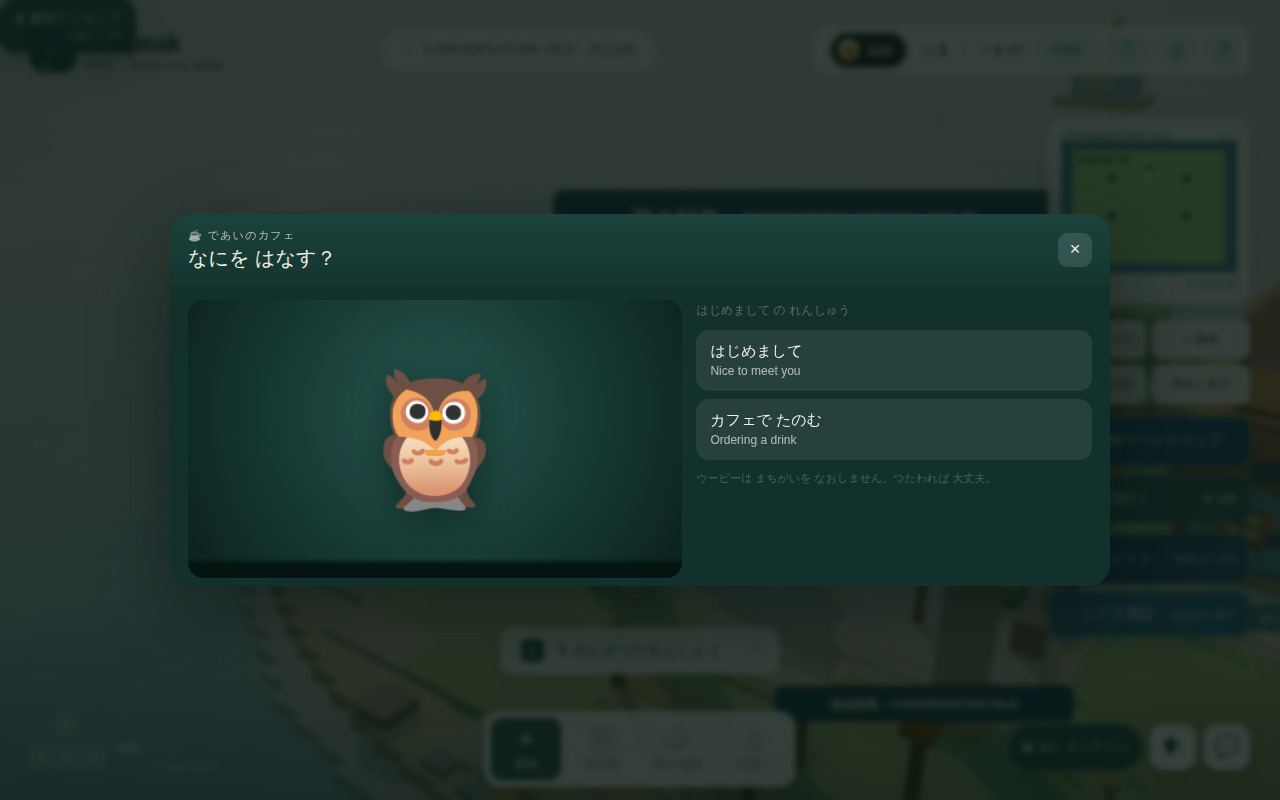
\includegraphics[width=4.9cm]{screen-conv.jpg}};
  \node[anchor=north west] at ($(current page.north west)+(12.6,-21.4)$)
    {
\includegraphics[width=4.9cm]{game-blockwild.jpg}};
  \node[anchor=north west, text=uspeakMint, font=\footnotesize, align=left]
    at ($(current page.north west)+(2.0,-24.7)$)
    {英検の島　　　　　　　　　　　AI英会話（キャラクター動画）　　　　同梱の別ゲーム};
  \node[anchor=south west, text=uspeakCream, font=\small, align=left]
    at ($(current page.south west)+(2.0,2.2)$)
    {ブラウザで URL を ひらくだけ。インストールも アカウントも いりません。};
  \node[anchor=south west, text=uspeakMint, font=\footnotesize]
    at ($(current page.south west)+(2.0,1.6)$) {2026年9月 ・ U-Speak Lab};
\end{tikzpicture}
\clearpage

% =================================================================== はじめに
\section{この資料について}

U-Speak Lab の英語学習ワールドを、\textbf{ブラウザで動くウェブ版}として作り直しました。
この資料は、\textbf{いま U-Speak Roblox を教室で使っていただいている先生}に向けて、
「どの島で・何を・どうやって学ぶのか」を、実際の画面とともに1つずつ説明するものです。

\begin{diffbox}
\textbf{いちばん大きな3つの違い}
\begin{enumerate}[leftmargin=18pt, itemsep=2pt]
  \item \textbf{インストールも アカウントも いりません。} 教室の iPad で URL を開けば、その場で始まります。
        Roblox アプリの更新待ちも、Roblox アカウントの管理も、年齢制限の確認もありません。
  \item \textbf{学習の記録を こちらが 持っています。} 何を何問正解したか、何を英語で話したかは
        すべてサーバーが確定し、Google スプレッドシートに入ります。先生はその場で開けて、
        保護者にはリンクか A4 の PDF でそのまま渡せます。
  \item \textbf{英検の島と、顔を見て話せる通話が あります。} 5級・4級・3級の4技能＋面接練習、
        そして世界の中で最大100人が話せる通話。どちらも Roblox 版にはなかったものです。
\end{enumerate}
\end{diffbox}

\subsection{ひと目で見る対照表}

\begin{center}
\footnotesize
\begin{tabular}{@{}p{0.19\textwidth} p{0.36\textwidth} p{0.39\textwidth}@{}}
\toprule
 & \textbf{U-Speak Roblox} & \textbf{U-Speak ウェブ版} \\
\midrule
はじめかた & Roblox アプリのインストール、Roblox アカウント、PlaceId & \textbf{URL を開くだけ}。クラスコードと名前を入れて参加 \\
端末 & Roblox が動く端末 & iPad / Chromebook / PC のブラウザ。教室の iPad で確認済み \\
教室での人数 & Roblox のサーバー任せ & \textbf{1クラス＝1ルーム}（既定30人）。1ワールド100人も実測済み \\
先生の操作 & なし & \textbf{先生コンソール}：全員集合・個別移動・呼び出し・チャット一時停止 \\
学習の記録 & DataStore ＋ シート同期 & Google スプレッドシートに直接。先生がその場で開ける \\
保護者へ & QRコードでレポート & リンクを配るだけ。さらに \textbf{A4 2ページの PDF} をその場で生成 \\
英検 & なし & \textbf{5級・4級・3級の島}。読む・聞く・書く・話す＋面接の間 \\
AI英会話 & チャット欄 & \textbf{キャラクターの動画つき}。声で話し、島の4場面＋おつかい島10か所 \\
通話 & Roblox のボイスチャット頼み & 世界の中で顔を見て話せる。おはなし島は\textbf{最大100人} \\
安全 & Roblox の TextService & 定型フレーズ＋自前のNGワード表。先生がチャットを止められる \\
課金 & Robux が世界の中にある & \textbf{世界の中にお金の入口はありません}。教室の月額のみ \\
ひとりのとき & 常にオンライン & \textbf{オフライン1人用モード}がそのまま残っています \\
\bottomrule
\end{tabular}
\end{center}

\begin{notebox}
\textbf{Roblox 版を否定する資料ではありません。} XP の伸び方（次のレベルまで ＝ 20＋レベル×10）、
コインの配り方、AI の人格「ウーピー」、夜のおばけ、乗り物の解放条件といった\textbf{設計の中身は
Roblox 版から そのまま移して}います。子どもから見れば同じ世界の続きです。
変わったのは、それを\textbf{どこで動かし、記録をだれが持つか}です。
\end{notebox}

\clearpage

% =================================================================== 地図
\section{世界の地図：14 の島}

空から降りて、行きたい島へ飛びます。島はどれも独立していて、順番はありません。

\begin{center}
\footnotesize
\begin{tabular}{@{}p{0.26\textwidth} p{0.30\textwidth} p{0.38\textwidth}@{}}
\toprule
\textbf{島} & \textbf{何をするところか} & \textbf{中身} \\
\midrule
はじまりの島 & 釣り・宝さがし・夜のおばけ & 魚100種（1匹＝英単語1つ）、RPG地域10、おばけ12種 \\
おつかい島 & 歩いて回る AI 英会話 & 店10か所、おつかい15件、段階式の会話 \\
ことばの学校島 & 単語クイズと 聞く・話すジム & \textbf{1{,}501問}、3段階の小屋＋ジム110語 \\
えいごアリーナ島 & 英語で戦うバトル & \textbf{249問}、CPU3段階＋たいせん台＋おさかな道場 \\
ペット島 & たまご・ごはん・ふれあい & 巣・ごはん処・ふれあい広場 \\
のりもの島 & 乗り物を買って レース & 4台（\coin{}100〜3000・Lv1〜10）、3周のレース \\
まちづくり島 & ブロックで 建てる & ブロック10種、かぐ11種、マイルーム、ひろば \\
英検5級の島 & 5級の 4技能 ＋ 面接 & よむ・きく・かく・はなす・めんせつの間 \\
英検4級の島 & 4級の 4技能 ＋ 面接 & 同上（問題は4級のもの） \\
英検3級の島 & 3級の 4技能 ＋ 面接 & 同上（問題は3級のもの） \\
英会話島 & ウーピーと 話す & カフェ・おかいもの・がっこう・とうだいの4場面 \\
おはなし島 & 人どうしが 話す & 4つの部屋。最大100人の通話 \\
きせかえ島 & アバターの 店 & 4つの店・\textbf{41点}（\coin{}40〜600） \\
ミニゲーム島 & 別ゲーム 2本の 家 & PUYO U-SPEAK ／ えいご スイカゲーム \\
テーマパーク & 遊具と ミニゲーム & 島ではなく、はじまりの島から入る区画 \\
\bottomrule
\end{tabular}
\end{center}

\subsection{どうやって 島へ 行くのか}

\shot{screen-map.jpg}{ワールドマップ。行き先を選んで飛びます。先生は全員をまとめて動かせます。}

\textbf{行き先を選んで、飛ぶだけです。} 島に順番はなく、授業でやりたい島へまっすぐ行けます。
RPGの10地域だけは物語と仲間集めで少しずつ開いていきますが、\textbf{学習の島は最初から
全部あいています}。先生コンソールからは、クラス全員を一度に同じ島へ動かせます。

\begin{notebox}
\textbf{時間は世界のもので、端末のものではありません。} 空は 昼300秒 → 夕方120秒 → 夜240秒 →
朝45秒 の11分45秒でめぐります。これは計算だけで決まるので、\textbf{同じ教室の全員が
いつでも同じ空の下}にいます。45分の授業なら3〜4回、日が暮れます。
\end{notebox}

\clearpage
% =================================================================== 島ごと
\section{島ひとつずつ}

\islandhead{はじまりの島}{WILLOW ISLAND}{最初に降りる島。釣り、宝さがし、10のRPG地域、そして夜。}
\shotw{0.62}{island-willow.jpg}{はじまりの島。桟橋で釣り、奥の道が10のRPG地域へ続く。}

\textbf{釣りが そのまま 単語学習です。} 魚は100種で、\textbf{1匹が英単語1つ}になっています
（名前・意味・級つき）。釣り上げると図鑑に載り、初めての魚はボーナス。買取屋で売ればコインになり、
魚によっては「わざ」を覚えます。宝箱と鍵の祭壇、そして10のRPG地域への入口もここです。

\textbf{夜になると おばけが出ます。} 12種。杖でふれるとキラキラ弾けてコインを落とします
（1日の上限つき）。夜は世界共通なので、\textbf{クラス全員に同時に}やってきます。

\begin{diffbox}
\rb{魚は実在の魚100種で、英語はついていませんでした。}
{\textbf{魚1匹＝英単語1つ}に作り直しました。釣ること自体が学習になります。
おばけは Roblox 版の仕組み（湧き方・コイン・1日の上限）をそのまま移し、
叩く手段は\textbf{杖だけ}に一本化しました（銃は移していません）。}
\end{diffbox}


\subsection{この島の画面}

\shotaside{screen-fishing.jpg}{英単語釣り。釣り場が英検の級で分かれている。}
{釣りはこの島のどこからでも開きます。釣り場を選び、ウキが沈んだら\textbf{その魚の英単語の
意味を当てる}。当たれば釣れて、図鑑に載ります。チャンスは2回、時間制限はありません。

釣った魚は\textbf{買取屋で売ってコイン}にでき、魚によっては「わざ」を覚えて
えいごアリーナ島の戦いで使えます。}

\facts{桟橋（釣り）・宝箱3か所・鍵の祭壇・10のRPG地域への入口・テーマパークのゲート}{魚1匹が英単語1つ（名前・意味・英検の級つき）。RPG地域の仲間も英語で捕まえる}{釣った種類、図鑑の埋まり具合、倒したおばけ、得たコインと XP}

\clearpage

\islandhead{おつかい島}{ERRAND ISLAND}{歩いて店を回り、店員と英語で話して用事をすませる。}
\shotw{0.62}{island-errand.jpg}{おつかい島。10軒の店と広場。用事のある店に矢印が出る。}

パン屋、港、森、雑貨屋、宿、図書館、博物館…\textbf{10か所を歩いて回ります}。
おつかいは15件あり、それぞれが\textbf{段階（ステージ）}に分かれています。
「パン屋で3個ください」を英語で言えたら次の段階、という進み方です。

店員との会話は\textbf{AIが相手}です。子どもは決まった文を選ぶこともできますし、
自分で打つ・話すこともできます。ヒントは日本語で出ます。

\begin{diffbox}
\rb{AI英会話はチャット欄にありました。相手は Emma / Oliver / Luna / Finn。}
{\textbf{島を歩いて店に入る}形にしました。用事のない店では会話が始まりません
（サーバーが位置を見ています）。AI の人格は Roblox 版の\textbf{「ウーピー（Upee・フクロウ先生）」に統一}し、
店員はウーピーが演じている役、という扱いです。
「あなたは AI ですか」と聞かれたときの答え方も Roblox 版から移しています。}
\end{diffbox}


\subsection{この島の画面}

\shotaside{screen-errand.jpg}{おつかいの一覧。15件が英検の級で分かれている。}
{広場で用事を受け取り、\textbf{その店まで自分で歩いて}行きます。
店に着くと店員との会話が始まり、\textbf{英語で用事をすませる}と次の段階に進みます。

決まった文から選んでも、自分で打っても、声で言ってもかまいません。
返事は英語、ヒントは日本語で出ます。}

\facts{パン屋・港・森・雑貨屋・宿・図書館・博物館など10か所}{店員との会話そのもの。選んで答えても、自分で打っても、声で言ってもよい}{おつかいの達成件数、話した回数、覚えた語}

\clearpage

\islandhead{ことばの学校島}{WORD SCHOOL}{単語クイズの小屋3つと、聞く・話すジム。}
\shotw{0.62}{island-school.jpg}{ことばの学校島。やさしい／ふつう／むずかしいの小屋と、奥にジム。}

\textbf{小屋に入ることが、難易度を選ぶことです。} やさしい小屋・ふつうの小屋・むずかしい小屋の
3軒があり、入った小屋の問題が10問出ます。問題は全部で\textbf{1{,}501問}。

\textbf{ことばのジム}では、聞こえた英語を選び、声に出して言います（110語）。
発音は端末の音声認識で拾い、\textbf{正誤はサーバーが決めます}。

\begin{notebox}
\textbf{問題文はブラウザに渡していません。} 1{,}501問はサーバーの中にあり、
子どもの画面には\textbf{いま出ている1問だけ}が届きます。
答え合わせもサーバーです（ブラウザは「どの問題にどの選択肢を答えたか」だけを送ります）。
だから、ページを覗いて答えを先に読むことはできません。
\end{notebox}


\subsection{この島の画面}

\shottwo{screen-quiz.jpg}{小屋の中。4択の単語クイズが10問。}{screen-gym.jpg}{ことばのジム。聞いて、声に出して言う。}

\vspace{2pt}
\small まちがえた問題はあとでもう一度出ます。ジムは端末の音声認識で声を拾いますが、
\textbf{合っているかどうかを決めるのはサーバー}です。\normalsize

\facts{やさしい小屋・ふつうの小屋・むずかしい小屋・ことばのジム}{4択の単語クイズ1{,}501問と、聞いて声に出す110語}{何問中何問、難易度ごとの正解率、語彙と聞く・話すの技能値}

\clearpage

\islandhead{えいごアリーナ島}{WORD ARENA}{英語でダメージを買う、バトルの島。}
\shotw{0.62}{island-arena.jpg}{えいごアリーナ島。3つの CPU 台と、たいせん台、おさかな道場。}

\textbf{攻撃は英語で買います。} 出題に正解するとダメージが出る、という戦い方です。
CPU は\textbf{らくらく・ふつう・つよい}の3段階。問題は\textbf{249問}。
勝てば XP とコイン。1日にもらえるコインには上限があります。

\textbf{おさかな道場}では、釣った魚から「わざ」を覚えます。図鑑と戦いがつながっている場所です。
\textbf{たいせん台}は子ども同士の対戦用に用意してあります。

\begin{diffbox}
\rb{アリーナと わざ習得は 別々の仕組みでした。}
{\textbf{同じ島の中}に置いて、釣り → 図鑑 → わざ → バトル が
歩いてつながるようにしました。ダメージ計算・勝敗・報酬はすべてサーバーが決めます。}
\end{diffbox}


\subsection{この島の画面}

\shotaside{screen-battle.jpg}{バトル。正解がそのまま攻撃になる。}
{相手の体力を削るには英語を当てるしかありません。難易度は入った台で決まり、
らくらく・ふつう・つよいの3段階。

勝ち負け、何問中何問、もらえるコインは\textbf{すべてサーバーが決めます}
（コインには1日の上限があります）。}

\facts{らくらく台・ふつう台・つよい台・たいせん台・おさかな道場}{正解がそのまま攻撃になる249問。わざの名前も英語}{勝敗、何問中何問、得たコイン（1日の上限つき）}

\clearpage

\islandhead{ペット島}{PET ISLAND}{たまごをもらい、かえして、育てる。}
\shotw{0.62}{island-pet.jpg}{ペット島。たまごの巣、ごはん処、ふれあい広場。}

\textbf{たまごの巣}でたまごをもらい、\textbf{ごはん処}でごはんをあげ、
\textbf{ふれあい広場}でなでます。空腹は時間で進みます。
ペットは世界の中を一緒についてきます。

英語との関わりは「世話をする理由」としてです。ごはんもなでる回数も、
コインと日課（デイリー）につながっています。

\begin{diffbox}
\rb{ペットの状態は DataStore に持っていました。}
{同じ項目を\textbf{スプレッドシートの列}に移しました。
どちらの端末から入っても、同じ子には同じペットがついてきます。}
\end{diffbox}


\subsection{この島の画面}

\shotaside{screen-pet.jpg}{たまごの巣。もらう・かえす・育てる。}
{たまごをもらい、ごはんをあげ、なでる。空腹は時間で進むので、
\textbf{次に来る理由}になります。

ペットは世界の中をついてきて、クラスの他の子からも見えます。
状態はサーバーが持っているので、どの端末から入っても同じ子がいます。}

\facts{たまごの巣・ごはん処・ふれあい広場}{ペットとお世話の言葉。日課（デイリー）とつながっている}{ペットの種類と状態、世話した回数}

\clearpage

\islandhead{のりもの島}{RIDE ISLAND}{乗り物を買って、3周のレースに出る。}
\shotw{0.62}{island-ride.jpg}{のりもの島。4つのゲートと、スタート・ゴールのライン。}

\textbf{乗り物は4台}。キックボード（\coin{}100・Lv1）、じてんしゃ（\coin{}400・Lv3）、
カート（\coin{}1{,}200・Lv6）、ホバーボード（\coin{}3{,}000・Lv10）。
\textbf{買えるのは、その乗り物のゲートまで歩いて行ったときだけ}です（サーバーが位置を見ています）。
買うと、その乗り物の英単語を1つ覚えます。

\textbf{スタート・ゴール}に立つと、島のコースを\textbf{3周}するレースが始まります。
順位・ラップ・ベストタイムはサーバーが判定します。クラスの誰かと一緒に走れます。

\begin{diffbox}
\rb{乗り物は Roblox の物理エンジン（VehicleSeat）で動いていました。}
{物理は再現していませんが、\textbf{見た目・値段・解放レベル・英単語}は
そのまま移しました。そのうえで\textbf{順位のあるレース}を足しています。}
\end{diffbox}

\subsection{この島の画面}

\shottwo{screen-garage.jpg}{ガレージ。値段・必要レベル・足りないコインが出る。}{screen-race.jpg}{レース本番。順位・ラップ・タイム。}

\vspace{2pt}
\small 買えないときは\textbf{なぜ買えないかが数字で出ます}（「あと \coin{}300」「あと Lv.2」）。
レースはこの島のコースを3周。\textbf{順位もラップも、判定はサーバー}です。\normalsize

\facts{キックボード置き場・じてんしゃ屋・カート工場・ホバー研究所・スタート・ゴール}{乗り物1台につき英単語1つ（kickboard / bicycle / kart / hoverboard）}{持っている乗り物、ベストラップ、レースの順位}

\clearpage

\islandhead{のりもの島・もうひとつのレース}{AURORA KART · ZENITH EDITION}{同じスタートラインから入る、まったく別のゲーム。}
\shotw{0.86}{game-racers.jpg}{AURORA KART。コーラル・コーストを8台で走っているところ。3周。}

\textbf{スタート・ゴールに立つと出るパネルの、いちばん上の扉}から入ります。
島のレースとは\textbf{別に作られたカートレース}を、1バイトも書き換えずにそのまま置いてあります。

\begin{center}
\small
\begin{tabular}{@{}p{0.26\textwidth} p{0.68\textwidth}@{}}
\toprule
コース & 4本（コーラル・コースト／サンセット・メサ／スターライト・パス／エンバー・フォージ） \\
マシン & 4台。最高速・加速・旋回がそれぞれ違う \\
遊び方 & レース・グランプリ・タイムアタック・\textbf{えいごモード} \\
戻り方 & 画面のメニューの「← U-Speak」。立っていた場所に戻ります \\
\bottomrule
\end{tabular}
\end{center}

\begin{diffbox}
\textbf{このゲームでは コインも 学習の記録も 動きません。}
正誤を判定しているのがそのゲーム自身（＝子どもの端末）だからです。
\textbf{遊びの時間として置いてあります。} 学習として数えるのは島の中の画面だけです。
\end{diffbox}

\clearpage

\islandhead{まちづくり島}{TOWN ISLAND}{ブロックを買って、部屋と ひろばに 建てる。}
\shotw{0.62}{island-town.jpg}{まちづくり島。ブロック屋、ふどうさん、かぐ屋、マイルーム入口、ブロックのとびら、ひろば。}

建てる場所は2つに分けてあります。\textbf{マイルーム}は自分だけの部屋（かぐ11種）、
\textbf{ひろば}はクラス全員で1つの世界を作る場所（ブロック10種）。

\textbf{ブロック屋}でブロックを買います。き（無料）から はじまって、
いし\coin{}30、レンガ\coin{}60、ガラス\coin{}90、ゆき\coin{}120、はな\coin{}150、
ランプ\coin{}200、みず\coin{}250 まで。
\textbf{どのブロックも、名前が英単語です}（wood / stone / brick / glass / lamp / water …）。
買った持ち物はサーバーが持っています。

\begin{diffbox}
\rb{建築は1つの世界で、同期と保存がいちばん重い機能でした。}
{\textbf{部屋（かぐ）と ひろば（ブロック）に分けました。}
部屋は一人ずつのインスタンス、ひろばはクラス共有。
どちらもサーバーが持ち主と中身を持っています。}
\end{diffbox}

\subsection{この島の画面（お店）}

\shottwo{screen-blockshop.jpg}{ブロック屋。10種が 3D のプレビューつきで並ぶ。}{screen-furniture.jpg}{かぐ屋。部屋に置くものが11種。}

\facts{ブロック屋・ふどうさん・かぐ屋・マイルーム入口・ブロックのとびら・ひろば}{ブロックとかぐの名前がすべて英単語（wood / stone / lamp / sofa …）}{買ったブロックとかぐ、建てたもの（部屋とひろば）}

\clearpage

\islandhead{まちづくり島・建てているところ}{TOWN ISLAND · BUILDING}{買ったものを、部屋と ひろばに 置く。}

\shottwo{screen-myroom.jpg}{マイルーム。自分だけの部屋に かぐを置く。}{screen-plaza.jpg}{ひろば。クラス全員で ひとつの世界を積む。}

\vspace{4pt}
\textbf{入口に歩いて入るだけで中に入れます。} メニューはありません。
画面中央の十字（＋）でねらって、\textbf{おく}（E）・\textbf{かたづけ}（Q）・
\textbf{むき}（R で90度）。手に持つものは下のバーか数字キー 1〜9 で選びます。

\textbf{マイルームは一人ずつ}、\textbf{ひろばはクラス共有}です。
ひろばに積んだブロックは他の子の画面にもその場で現れ、次の授業にも残っています。
どちらも\textbf{中身を持っているのはサーバー}なので、端末が変わっても同じ部屋に入れます。

\subsection{この島から入る、別のゲーム}

\shotaside{game-blockwild.jpg}{BLOCKWILD の世界の中。下のバーにあるのは き だけ。}
{島に建っている\textbf{「ブロックの とびら」という建物}に歩いて入ります。
ブロックを積んで世界を作る、\textbf{まったく別のゲーム}です。

\textbf{ここが ブロック屋と つながっています。} クリエイティブで手に持てるのは、
\textbf{ブロック屋で U-Speak コインを払って買ったブロックだけ}。写真の下のバーに
き（wood）しか入っていないのは、この子がまだ何も買っていないからです。
英語をやってコインを稼ぐと、建てられるものが増えます。

「← U-Speak」で島に戻ります。\textbf{コインも学習の記録も動きません}。}

\clearpage

\islandhead{英検5級の島}{EIKEN 5 · STARTER ISLE}{読む・聞く・書く・話す、そして面接。Roblox 版にはなかった島です。}
\shotw{0.62}{island-eiken5.jpg}{英検5級の島。よむ図書館・きく音楽堂・かく工房・はなすステージ・めんせつの間。}

\textbf{建物が そのまま 技能です。}

\begin{center}
\small
\begin{tabular}{@{}p{0.26\textwidth} p{0.30\textwidth} p{0.34\textwidth}@{}}
\toprule
\textbf{建物} & \textbf{技能} & \textbf{1級あたりの問題} \\
\midrule
よむ図書館 & Reading（読む） & 10問 \\
きく音楽堂 & Listening（聞く） & 12問 \\
かく工房 & Writing（書く） & 12問 \\
はなすステージ & Speaking（話す） & 10問 \\
めんせつの間 & 二次試験の練習 & カード2枚 \\
\bottomrule
\end{tabular}
\end{center}

島は\textbf{5級・4級・3級の3つ}あります（4級の島も同じ作りです）。
どの級のどの技能も、\textbf{正誤はサーバーが判定}し、マイページの5技能グラフに積まれます。

\begin{notebox}
\textbf{めんせつの間}は二次試験のかたちをそのままなぞります。
カードの絵を見て、パッセージを音読し、質問に答え、最後に自分のことを聞かれます。
面接官はキャラクターの動画で、待ち時間も本番と同じように進みます。
\end{notebox}


\subsection{この島の画面}

\shottwo{screen-eiken.jpg}{よむ図書館。級と技能は建物で決まっている。}{screen-interview.jpg}{めんせつの間。面接官はキャラクター。}

\facts{よむ図書館・きく音楽堂・かく工房・はなすステージ・めんせつの間}{英検5級の4技能。読む10・聞く12・書く12・話す10、面接カード2枚}{級ごと・技能ごとの正解率。マイページの5技能グラフに積まれる}

\clearpage

\islandhead{英検3級の島}{EIKEN 3 · VOYAGER ISLE}{同じ5つの建物で、中身が3級。}
\shotw{0.62}{island-eiken3.jpg}{英検3級の島。島の色と地形が級ごとに違うので、どこにいるか一目でわかる。}

5級・4級・3級で\textbf{建物の並びは同じ}にしてあります。
「よむ図書館は左手前」が3つの島で共通なので、級が上がっても迷いません。
\textbf{違うのは中身だけ}です。

3級の書く問題には英作文が入り、面接カードの質問も長くなります。
どこまで進んだかは級ごとに別々に記録されるので、
「5級は終わったが4級はこれから」という状態がそのまま残ります。


\subsection{この島の画面}

\shotaside{screen-eikenwrite.jpg}{3級の「かく」。英作文が入ります。}
{5級・4級と同じ5つの建物ですが、中身は3級です。
書く問題には\textbf{英作文}が入り、面接カードの質問も長くなります。

\textbf{記録は級ごとに別々}なので、「5級は終わったが4級はこれから」
という状態がそのまま残ります。どの級から受けてもかまいません。}

\facts{5級・4級の島と同じ並びの5つの建物}{英検3級の4技能（書くには英作文が入ります）と、長めの面接}{級ごとに別々。5級が終わっていなくても3級を受けられる}

\clearpage

\islandhead{英会話島}{CONVERSATION ISLE}{ウーピーと、場面を決めて話す島。}
\shotw{0.62}{island-conv.jpg}{英会話島。であいのカフェ、おかいものストリート、がっこうテラス、ゆめのとうだい。}

\textbf{場所が場面です。} であいのカフェ（はじめまして）、おかいものストリート（買い物）、
がっこうテラス（学校のこと）、ゆめのとうだい（将来の夢）。
入った建物で、話す話題が決まります。

相手は\textbf{キャラクターの動画}で出ます。声で話しかけても、打ち込んでもかまいません。
返事は英語、ヒントは日本語。話した回数と内容の要約は記録に残ります
（\textbf{話した文そのものは 保護者レポートには載せません}）。

\begin{diffbox}
\rb{AI との会話はチャット欄で、相手の顔はありませんでした。}
{\textbf{顔のあるキャラクターと、島の場面}にしました。
1日に話せる時間には上限を入れてあります（費用と、使いすぎの両方のために）。}
\end{diffbox}


\subsection{この島の画面}

\shottwo{screen-conv.jpg}{入った建物で、話す場面が決まる。}{screen-convtalk.jpg}{ウーピーと話しているところ。}

\vspace{2pt}
\small 声で話しても、打ち込んでもかまいません。返事は英語、ヒントは日本語。
「もう一度」ボタンで聞き直し、「ヒント」ボタンで言い方を教えてくれます。\normalsize

\facts{であいのカフェ・おかいものストリート・がっこうテラス・ゆめのとうだい}{ウーピーとの自由な会話。入った建物が話題を決める}{話した回数と時間（1日の上限つき）。話した文そのものは保護者に出しません}

\clearpage

\islandhead{おはなし島}{TALK ISLAND}{人どうしが、顔を見て話す島。}
\shotw{0.62}{island-talk.jpg}{おはなし島。おしゃべりブース、しずかなブース、はっぴょうルーム、せんせいルーム。}

\textbf{部屋に入ると、その部屋の人と通話がつながります。} カメラとマイクは自分で選べます。
4つの部屋があり、\textbf{はっぴょうルーム}は発表用、\textbf{せんせいルーム}は先生を呼ぶ用です。

\textbf{最大100人}。教室全員を1つの部屋に入れて、朝の会や発表会に使えます。
（100人の通話には LiveKit の設定が要ります。未設定なら6人までのメッシュ通話になります。）

\begin{notebox}
\textbf{通話にも1日の上限があります。} 1人あたりの分数をサーバーが数えていて、
上限に達すると通話だけが止まります（世界には残れます）。
AI英会話と同じ考え方です。
\end{notebox}


\subsection{この島の画面}

\shotaside{screen-talk.jpg}{部屋に入ると出る通話のパネル。}
{\textbf{部屋に入ることが、通話に入ることです。} マイクとカメラはそれぞれ切れます。
文字でも書けるので、声を出しにくい子も参加できます。

先生は\textbf{せんせいルーム}に入って呼び出しに答えられます。
通話できる島は先生コンソールから絞れます。}

\facts{おしゃべりブース・しずかなブース・はっぴょうルーム・せんせいルーム}{人どうしの会話。先生が入って課題を出すこともできる}{通話した時間（1日の上限つき）}

\clearpage

\islandhead{きせかえ島}{DRESS-UP ISLE}{4つの店で、アバターの見た目を買う。}
\shotw{0.62}{island-wear.jpg}{きせかえ島。ぼうしや・めがねや・かばんや・アクセサリーや、そして広場の鏡。}

\textbf{店が そのまま スロットです。} ぼうしや（頭）、めがねや（顔）、かばんや（背中）、
アクセサリーや（むね）。入った店の品物がそのまま開きます。

品物は\textbf{全部で41点}（帽子11・顔10・背中10・むね10）、\coin{}40 から \coin{}600。
どれも\textbf{メニューの中で 3D で回って見えます}。買う前に、実際にどう見えるかがわかります。

着たものは\textbf{クラスの全員から見えます}。誰が何を着ているかは、その場の全員の画面に届きます。
きせかえはヘッダーの きせかえボタンからどこでも開けます。島は「買いに行く楽しみ」のほうです。

\begin{diffbox}
\rb{きせかえは Roblox の Shirt / Pants アセットと InsertService を使っていました。}
{\textbf{アバターを作り直し}、41点をこちらのデータとして持っています。
持ち物はサーバーのもの、値段もサーバーが決めます。}
\end{diffbox}


\subsection{この島の画面}

\shottwo{screen-wardrobe.jpg}{ぼうしや。11点。}{screen-wearback.jpg}{かばんや。せなかに着けるもの10点。}

\vspace{2pt}
\small \textbf{カードの中の品物は 3D で回っています。} 買う前に、実際にどう見えるかがわかります。
着たものはクラス全員の画面に届きます。\normalsize

\facts{ぼうしや・めがねや・かばんや・アクセサリーや}{品物の名前が英単語。買うとその語を覚える}{持っている品と、いま着ているもの（クラス全員から見えます）}

\clearpage

\islandhead{ミニゲーム島}{MINIGAME ISLE}{家が2軒。それぞれが 別のゲーム。}
\shotw{0.62}{island-mini.jpg}{ミニゲーム島。左の家が PUYO U-SPEAK、右の家が えいご スイカゲーム。}

この島には\textbf{家が2軒しかありません}。名前の書いてあるほうの家に入ると、
そのゲームが全画面で始まります。どちらも英単語を使ったパズルです。

\begin{itemize}[leftmargin=16pt, itemsep=1pt]
  \item \textbf{PUYO U-SPEAK} — ぷよを消しながら英単語を作るゲーム。
  \item \textbf{えいご スイカゲーム} — 同じものどうしを合体させていくゲーム。英単語つき。
\end{itemize}

どちらも\textbf{別に作られたゲーム}で、この世界のコードとは独立しています（詳しくは後述）。
「← U-Speak」を押せば島に戻ります。


\subsection{この島の画面}

\shottwo{game-puyo.jpg}{PUYO U-SPEAK。ぷよを消して英単語を作る。}{game-suika.jpg}{えいご スイカゲーム。同じものを合わせていく。}

\facts{左の家＝PUYO U-SPEAK、右の家＝えいご スイカゲーム}{どちらのゲームも英単語を作る／合わせるルール}{\textbf{残りません。}遊びの時間として置いてあります}

\clearpage

\islandhead{テーマパーク}{WONDER PARK}{遊具と ミニゲームの区画。}
\shotw{0.62}{island-park.jpg}{テーマパーク。はじまりの島のゲートから入る。}

観覧車、コーヒーカップ、ミニゲーム。\textbf{英語の課題がない場所}です。
授業の切れ目に、あるいは早く終わった子の待ち時間に使えます。

置いてある理由は1つです。\textbf{ずっと勉強している世界には、子どもは長く居ません。}
釣り、ペット、レース、きせかえ、テーマパークは、
「また来たい」と思うための場所として意図的に置いてあります。

\begin{notebox}
\textbf{遊びの場所にも、上限はあります。} 世界の中にお金の入口はないので、
ここで遊ぶために何かを買わせることはありません。コインは英語をやって得るものだけです。
先生コンソールからは\textbf{クラス全員を1か所に集められる}ので、
「そろそろ戻ろう」は1回の操作でできます。
\end{notebox}


\facts{観覧車・コースター・メリーゴーランド・ミニゲーム}{乗り物の名前は単語帳に入りますが、課題はありません}{\textbf{ほとんど残りません。}休むための場所です}

\clearpage
% =================================================================== 画面
\section{どの島からでも 開く画面}

島の中の画面は、それぞれの島のページに載せました。ここは\textbf{どこにいても開けるもの}です。

\subsection{マイページ（子どもが見る記録）}

\shot{screen-dashboard.jpg}{マイページ。5技能の伸びと、やったことの記録。}

\textbf{マイページ}は子ども自身が見る記録です。読む・聞く・書く・話す・語彙の5技能を、
やった量と正解率から出しています。\textbf{同じ数字}が保護者レポートにも出ます。

\subsection{先生コンソール}

\shot{screen-teacher.jpg}{先生コンソール。世界を見ながら、右のパネルで操作する。}

\textbf{講師キーを入れた人にだけ出ます。} 判定はサーバー側だけで行うので、
ブラウザをいじって先生になることはできません。

\begin{center}
\small
\begin{tabular}{@{}p{0.30\textwidth} p{0.64\textwidth}@{}}
\toprule
全員をここに集合 & クラス全員を、先生のいる場所へ呼びます \\
名簿から その子へ & 名前を押すと、その子のところへ飛びます \\
チャットを一時停止 & いますぐ全員のチャットを止めます \\
じゆうにゅうりょく & 自由入力を許すか、定型フレーズだけにするか \\
おはなし & 通話をどの島で許すか \\
今日のおつかい & クラス全員の課題をそろえます \\
保護者レポートのリンク & 一人ひとりのレポート URL を配ります（名簿の横のボタンから PDF も） \\
\bottomrule
\end{tabular}
\end{center}

\clearpage

% =================================================================== 記録
\section{記録と、保護者にお渡しするもの}

\begin{center}
\small
\begin{tabular}{@{}p{0.28\textwidth} p{0.66\textwidth}@{}}
\toprule
\textbf{渡すもの} & \textbf{中身} \\
\midrule
マイページ（子ども） & 5技能のグラフ、レベル、コイン、やったことの一覧 \\
レポートのリンク（保護者） & 一人ひとりのページ。先生コンソールから配れる \\
A4 2ページの PDF & 表紙にレベル・正解率・やったことの棒グラフ。2ページ目に全記録と「つぎのもくひょう」 \\
Google スプレッドシート & クラス全員分の生データ。先生がそのまま開いて並べ替えられる \\
\bottomrule
\end{tabular}
\end{center}

\subsection{A4 2ページの 保護者レポート}

\begin{center}
\shotpage{report-page1.jpg}{1ページ目。名前、3つのリング、やったことの棒グラフ、レベルの印。}
\hfill
\shotpage{report-page2.jpg}{2ページ目。ぜんぶの記録と「つぎの もくひょう」、数字の出どころ。}
\end{center}

\vspace{4pt}
先生コンソールのボタンひとつで出ます。教室で刷って、そのままお渡しできます
（\textbf{見本です。名前も数字も架空のものです}）。

\begin{notebox}
\textbf{書いた文や 話した内容は 保護者レポートに載せません。} 載せるのは学習の記録
（何を何問、正解率、レベル、やったこと）だけです。
数字は\textbf{画面と紙で同じもの}を使っています（1つの計算から両方を作っているため、食い違いません）。
\end{notebox}

\subsection{数字は だれが 決めているか}

\begin{center}
\small
\begin{tabular}{@{}p{0.42\textwidth} p{0.52\textwidth}@{}}
\toprule
\textbf{子どもの端末が決めていること} & \textbf{サーバーが決めていること} \\
\midrule
どこに立っているか、どちらを向いているか、走っているか歩いているか &
\textbf{正誤・XP・コイン・購入・持ち物・学習の記録・レベル・順位・先生かどうか} \\
\bottomrule
\end{tabular}
\end{center}

保護者にお見せする数字は、すべて右の列から出ています。
子どもの端末は「どの問題に、どの選択肢を答えたか」を送るだけで、\textbf{点数は送りません}。
\textbf{ブラウザの中をいじってコインを増やす、正解率を上げる、といったことはできません。}

\clearpage

% =================================================================== 同梱ゲーム
\section{同梱している 別のゲーム 4本}

島の中から、\textbf{まったく別に作られたゲーム}が4本開きます。
どれも全画面で始まり、「← U-Speak」で島に戻ります。写真は それぞれの島のページにあります。

\begin{center}
\small
\begin{tabular}{@{}p{0.30\textwidth} p{0.30\textwidth} p{0.34\textwidth}@{}}
\toprule
\textbf{ゲーム} & \textbf{どこから入るか} & \textbf{中身} \\
\midrule
AURORA KART & のりもの島・スタート・ゴールのパネル & 3Dカートレース。コース4本・グランプリ・タイムアタック・えいごモード \\
BLOCKWILD & まちづくり島・\textbf{ブロックの とびら}（歩いて入る建物） & ブロックの世界。クリエイティブとサバイバル \\
PUYO U-SPEAK & ミニゲーム島・左の家 & ぷよを消して英単語を作るパズル \\
えいご スイカゲーム & ミニゲーム島・右の家 & 同じものを合わせていくパズル。英単語つき \\
\bottomrule
\end{tabular}
\end{center}

\vspace{4pt}

\subsection{ブロック屋 と BLOCKWILD が つながっています}

BLOCKWILD は独立したサンドボックスですが、\textbf{そこで使えるブロックは、
まちづくり島のブロック屋で U-Speak コインを払って買ったものだけ}です。

\begin{center}
\small
\begin{tabular}{@{}l l l l l@{}}
\toprule
き \textit{wood} \coin{}0 & いし \textit{stone} \coin{}30 & レンガ \textit{brick} \coin{}60 & ガラス \textit{glass} \coin{}90 & くさ \textit{grass} \coin{}40 \\
すな \textit{sand} \coin{}40 & ゆき \textit{snow} \coin{}120 & はな \textit{flower} \coin{}150 & ランプ \textit{lamp} \coin{}200 & みず \textit{water} \coin{}250 \\
\bottomrule
\end{tabular}
\end{center}

つまり、\textbf{英語をやってコインを稼ぐと、建てられるものが増えます}。
持ち物はサーバーが持っているので、どの端末から入っても同じです。

\begin{notebox}
\textbf{4本とも、1バイトも書き換えずに置いてあります。} 元のファイルのハッシュを毎回照合していて、
違っていればテストが止まります。必要な手当て（つながらないオンライン機能を隠す、
帰り道のボタンを足す、買っていないブロックを出さない）は\textbf{外から}行っていて、
ゲーム本体には手を入れていません。だから作者のビルドを差し替えるだけで新しい版に上げられます。
\end{notebox}

\begin{diffbox}
\textbf{ご注意：この4本では コインも 学習記録も 動きません。}
正誤を判定しているのはそのゲーム自身（＝子どもの端末）なので、
保護者にお見せする数字には入れていません。\textbf{遊びの時間として置いてあります。}
学習として数えるのは、島の中の画面だけです。
\end{diffbox}

\clearpage
% =================================================================== 運用
\section{教室での 使い方}

\subsection{授業のはじめ}

\begin{enumerate}[leftmargin=18pt, itemsep=2pt]
  \item 子どもは iPad で\textbf{URL を開きます}（ホーム画面に置いておけば1タップ）。
  \item 名前を入れて、\textbf{クラスコード}を入れて「はじめる」。
  \item 先生は同じ画面で「先生用」を開き、\textbf{講師キー}を入れて参加します。
  \item 全員そろったら、先生コンソールの\textbf{「全員集合」}で1か所に集められます。
\end{enumerate}

インストールはありません。アカウントもありません。名簿と照合する\textbf{入場ゲート}を
有効にすれば、名簿にない名前は入れなくなります。

\subsection{何人まで入れるか（実測）}

\begin{center}
\small
\begin{tabular}{@{}p{0.42\textwidth} p{0.52\textwidth}@{}}
\toprule
\textbf{構成} & \textbf{結果} \\
\midrule
1クラス 25人 × 10分 & 下り 4.3 KB/s/台、遅延 p95 49 ms、切断 0 \\
4クラス × 25人（100人同時） & 下り 4.2 KB/s/台、遅延 p95 50 ms、切断 0 \\
1つの世界に 100人 & 下り 16 KB/s/台、遅延 p95 75 ms、切断 0 \\
教室のネット越しに 25人（実測） & 下り 3.8 KB/s/台、遅延 p95 182 ms、切断 0 \\
\bottomrule
\end{tabular}
\end{center}

ふだんは\textbf{1クラス＝1ルーム}で使い、学校全体のイベントのときだけ1つの世界にまとめます。
遠くの子は描画を間引くので、100人でも iPad の負担は変わりません。

\subsection{iPad で 困りやすいこと}

\begin{center}
\small
\begin{tabular}{@{}p{0.40\textwidth} p{0.54\textwidth}@{}}
\toprule
\textbf{起きること} & \textbf{どうなるか} \\
\midrule
ホームに戻って また開いた & \textbf{3秒以内に}元の場所へ戻ります（席は60秒とっておきます） \\
Wi-Fi が一瞬切れた & 自動でつなぎ直します。持ち物も進み具合もそのまま \\
ネットが完全に落ちた & ロビーの「ひとりで遊ぶ」で\textbf{オフラインでも遊べます} \\
画面が小さい端末 & 縦でも横でも組み直します（21画面 × 5サイズで確認済み） \\
\bottomrule
\end{tabular}
\end{center}

\subsection{お金と 安全について}

\begin{itemize}[leftmargin=16pt, itemsep=2pt]
  \item \textbf{世界の中に お金の入口はありません。} Robux にあたるものは作っていません。
        コインは英語をやって得るものだけです。
  \item \textbf{チャットは 定型フレーズが基本}です。自由入力もできますが、
        NGワード表を通し、\textbf{先生がいつでも止められます}。
  \item \textbf{AI英会話とビデオ通話には 1日の上限}があります（教室ごとに設定）。
  \item \textbf{鍵はブラウザに入っていません。} AI のキーも、通話のキーも、
        シートの鍵も、すべてサーバーの環境変数です。ページを保存しても出てきません。
  \item 通信は \textbf{wss://}（暗号化）です。
\end{itemize}

\clearpage

% =================================================================== 付録
\section{付録：数字の一覧}

\begin{center}
\small
\begin{tabular}{@{}p{0.40\textwidth} p{0.54\textwidth}@{}}
\toprule
\textbf{項目} & \textbf{数} \\
\midrule
島 & 14（＋テーマパークの区画） \\
単語クイズの問題 & 1{,}501問（やさしい／ふつう／むずかしい） \\
バトルの問題 & 249問 \\
ことばのジムの語 & 110語 \\
英検の問題 & 1級あたり44問（読10・聞12・書12・話10）× 5級・4級・3級 \\
英検の面接カード & 1級あたり2枚 × 3級 \\
おつかい & 15件・店10か所 \\
魚 & 100種（1匹＝英単語1つ） \\
夜のおばけ & 12種（1日のコイン上限つき） \\
乗り物 & 4台（\coin{}100〜3{,}000・Lv1〜10） \\
ブロック & 10種（\coin{}0〜250）／ かぐ 11種（\coin{}0〜800） \\
きせかえ & 41点・4スロット（\coin{}40〜600） \\
定型フレーズ & 5分類・36文 \\
同梱の別ゲーム & 4本 \\
レベル曲線 & 次のレベルまで ＝ 20 ＋ レベル × 10（Roblox 版と同じ式） \\
1日の空 & 昼300秒・夕方120秒・夜240秒・朝45秒（1周 11分45秒） \\
\bottomrule
\end{tabular}
\end{center}

\subsection{動かすのに 必要なもの}

\begin{center}
\small
\begin{tabular}{@{}p{0.28\textwidth} p{0.66\textwidth}@{}}
\toprule
子どもの端末 & 今どきのブラウザ（iPad Safari / Chrome / Edge）。インストール不要 \\
先生の端末 & 同じ。講師キーを入れると先生コンソールが出ます \\
ネット & 1台あたり 下り 4 KB/s ほど。教室の Wi-Fi で足ります \\
サーバー & こちらで用意します（東京リージョン）。学校に置く必要はありません \\
記録の置き場 & Google スプレッドシート（教室のものをお使いいただけます） \\
\bottomrule
\end{tabular}
\end{center}

\subsection{品質について}

このワールドは\textbf{自動テストで守られています}。
サーバーの判定・経済・出題、島の地形（立てる場所があるか、道が建物を貫いていないか、
扉が重なっていないか）、そして\textbf{実際のブラウザを動かす検査}（島を歩き、店で買い、
ゲームを開いて閉じる）を、変更のたびに全部走らせています。
同梱ゲームのファイルはハッシュで照合しているので、\textbf{中身が変わっていれば止まります}。

\vspace{10pt}
\begin{notebox}
\textbf{1か月の無料体験をご用意しています。} 教室のクラスコードをお作りして、
そのまま授業でお使いいただけます。記録もレポートも、体験中から本番と同じものが出ます。
\end{notebox}

\vspace{14pt}
\begin{center}
\color{uspeakGreen}\small
U-Speak Lab ／ この資料の画面はすべて、実際に動いているワールドから撮ったものです。
\end{center}

\end{document}
